\chapter{Proxy}
\label{proxy}
\section{Definici'on}

Los servidores proxy son intermediarios entre el cliente y el servidor. Act'uan enviando los mensajes del cliente al servidor y viceversa. En una comunicaci'on normal, le cliente se comunica directamente con el servidor, en el caso de que en la red haya un proxy presente, el cliente se comunica con el proxy y este es el que se comunica con el servidor.

El proxy HTTP es un web server y tambi'en es cliente. Para recibir los pedidos de los clientes, tiene que actuar como un servidor y manejar correctamente las peticiones, conexiones y respuestas. A su vez, para poder conectarse a los destinos finales y recuperar los recursos que le son pedidos por el usuario del proxy, tiene que actuar como un cliente, enviando peticiones y recibiendo las respuestas. Se puede ver el funcionamiento b'asico de un proxy en la Figura \ref{proxy_1}.

\begin{figure}[ht!]
  	\centering
	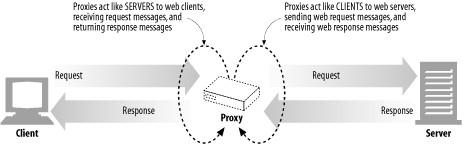
\includegraphics[width=310px]{img/proxy_1}
	\caption{\small Esquema del funcionamiento de un proxy, extra'ido de \cite{httpGuide}}
	\label{proxy_1}
\end{figure}

El esquema de la Figura \ref{proxy_1} muestra una conexi'on utilizando HTTP, las peticiones viajan directamente al proxy y de ah'i al servidor final. En el caso de HTTPS se hace de manera diferente. Primero el cliente env'ia una petici'on con el m'etodo CONNECT que incluye la direcci'on y el puerto del destino final. El proxy autentica la conexi'on, completa la negociaci'on con el destino y responde al cliente con un mensaje que contiene el c'odigo 200 que indica que la conexi'on fu'e establecida. Luego, el proxy se convierte en un t'unel que solo reenv'ia los paquetes del cliente hacia el servidor y viceversa (todo el tr'afico se encuentra encriptado). Esto puede ilustrarse en la Figura \ref{proxy_2}.
\label{mitm}
Los browsers actuales no soportan proxies HTTP Seguros, es decir, que se establezca una sesi'on SSL del cliente al proxy y otra del proxy al servidor final como puede verse en la Figura \ref{trustedProxy}. Este 'ultimo punto est'a en discusi'on, se propuso un borrador \citep{draftTrustedProxy} al respecto.

\begin{figure}[h]
  	\centering
	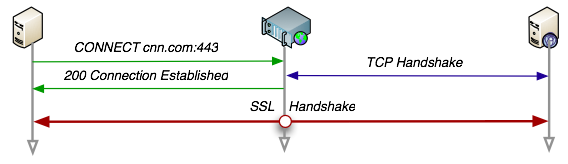
\includegraphics[width=\textwidth]{img/proxy_2}
	\caption{\small T'unel HTTPS sobre un proxy, extra'ido de \cite{secureProxies}}
	\label{proxy_2}
\end{figure}

\begin{figure}[h]
  	\centering
	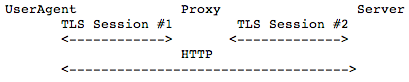
\includegraphics[width=\textwidth]{img/trustedProxy}
	\caption{\small T'unel HTTPS sobre un proxy, extra'ido de \cite{draftTrustedProxy}}
	\label{trustedProxy}
\end{figure}

\section{Usos de un Proxy}

Hay diversas utilizaciones de los servidores proxy, entre ellas se destacan:

\begin{enumerate}
\item Proxy NAT\footnote{Network Address Translation.} / Enmascaramiento

El enmascaramiento IP o tambi'en llamado traducci'on de direcciones de red, es el proceso por el cual las direcciones IP del origen/destino son reescritas, se sustituyen por otras. Es 'util cuando se dispone de una 'unica direcci'on p'ublica que se comparte entre varios usuarios. El proxy se encarga de enmascarar las direcciones privadas de los clientes, traduciendol'a a la direcci'on p'ublica, para realizar las peticiones al exterior. Cuando recibe la respuesta de los servidores exteriores, se encarga de derivarla al usuario que inici'o el pedido.

\item Filtro

El proxy al recibir las peticiones de los clientes, puede permitir o denegar esas peticiones seg'un ciertas pol'iticas definidas. Por ejemplo, en una Instituci'on Educativa se podr'ia bloquear el acceso a ciertas redes sociales o sitios para adultos.

\item Cortafuegos\footnote{Firewall.}

Al ser un intermediario, y muchas veces como puerta de acceso hacia internet, se pueden utilizar para aumentar el nivel de seguridad restringiendo ciertos protocolos o filtrando cierto contenido inseguro por ejemplo.

\item Web Cach'e

Puede utilizarse para mantener copias locales de los recursos peticionados por los clientes, y al momento de recibir una petici'on por un recurso que se encuentra almacenado, se brinda esa copia al cliente. Al servir varios clientes esto incrementa la velocidad de respuesta. Es uno de los usos m'as importantes de un proxy, ya que reduce notablemente los tiempos de carga de los sitios cuando se produce un cach'e hit. Esto se ver'a detalladamente en el Cap'itulo \ref{cache}.

\item Proxy Reverso / Surrogate Server

Puede actuar delante de un servidor web, atendiendo peticiones de los clientes como si fuera 'el servidor mismo. Esto permite por ejemplo, generar una red de distribuci'on de contenidos (CDN). Recibe una petici'on de un cliente, y, en vez de devolver el contenido directamente, inicia una comunicaci'on con otros servidores para localizar el recurso pedido, de manera m'as eficiente. Tambi'en protege a los servidores web, a'nadiendo una capa adicional de defensa. Puede distribuir la carga entre varios servidores web.

\item Content-Router

Pueden redirigir las peticiones a diferentes servidores, basados en las condiciones del tr'afico de Internet y el tipo de contenido.

\item Transcoder

Puede modificar el contenido de los recursos antes de hacer el env'io a los clientes. Por ejemplo, transformar im'agenes BMP a JPEG para reducir el tama'no, comprimir archivos de texto, e incluso hacer una traducci'on del contenido a otro lenguaje.

\item Anonimizador

Permite navegar de manera privada y an'onima removiendo ciertos datos de los mensajes HTTP (direcci'on IP, From header, cookies, etc).

\end{enumerate}

\section{Ventajas y Desventajas}

\subsection{Ventajas}

\begin{enumerate}
\item Control

Al ser intermediario, es el proxy el 'unico que va a realizar el trabajo de comunicaci'on hacia el exterior, es el que tiene la potestad de limitar y restringir los derechos de los clientes, ya que todo pasa a trav'es de 'el.
\clearpage
\item Optimizaci'on de los tiempos de carga

En el caso de los proxies que ofrecen servicio de cach'e, se optimizan los tiempos de carga de los sitios, al tener almacenada copias locales que puede brindar directamente al usuario sin tener que realizar la petici'on al servidor final.
\item Optimizaci'on del uso de recursos

El proxy es el 'unico que realiza el trabajo hacia afuera, es decir, que al utilizar una sola conexi'on, se maximiza el uso del ancho de banda.
\item Modificaci'on de la Informaci'on

Al tener acceso a los recursos que viajan a trav'es de 'el, tiene la posibilidad de modificarlos.
\item Filtrado

Recibir todas las peticiones del usuario, da la posibilidad de poder decidir que recursos o qu'e sitios son los que est'an habilitados para su recuperaci'on. Podr'ia manejarse una lista negra\footnote{Listado de sitios a los que NO se puede acceder.} o una lista blanca\footnote{Listado de sitios cuyo acceso est'a permitido.} por ejemplo.

\item Tr'afico controlado

Debido a que todo el tr'afico pasa a trav'es del proxy, se puede registrar un gran volumen de informaci'on que luego puede usarse para auditor'ia y seguridad.
\item Anonimato

Permite a los usuarios acceder a los servicios que brinda Internet, protegiendo la red interna. Al acceder al exterior identific'andose como el mismo, es dif'icil para el recurso diferenciar quien es el que est'a realizando la petici'on.
\end{enumerate}
\clearpage
\subsection{Desventajas}

\begin{enumerate}
\item M'ultiples funciones

Al estar a disposici'on de todas las peticiones de los usuarios, es posible que tenga que realizar algunas tareas no espec'ificas de su funci'on, por ejemplo los controles de acceso a sus servicios.
\item Carga de trabajo

Al ser el intermediario de todos los usuarios, el proxy tiene que realizar el trabajo de todos ellos. La carga de trabajo crece en la medida en que crezcan la cantidad de usuarios que consumen sus servicios.
\item Confianza del Usuario

Pueden aparecer usuarios que no se sientan c'omodos con que todo su tr'afico sea interceptado. Adem'as, todas las transacciones realizadas se guardan en archivos de logs\footnote{Registro oficial de eventos durante un rango de tiempo en particular.}, es decir que toda la actividad que el usuario realice a trav'es del proxy quedan registradas. En una conexi'on sin intermediarios, es imposible tener la informaci'on completa de las transacciones realizadas ya que se encuentra esparcida en servidores diseminados por todo el mundo.
\item Modificaci'on en el Software de los usuarios

La utilizaci'on de un proxy, requiere que las aplicaciones que interact'uan con Internet que los usuarios utilizan en la red interna, se configuren (ver Secci'on \ref{proxyConf}) para que puedan tener acceso hacia el exterior a trav'es del proxy. 
\item Servicios no disponibles

Existen algunos aplicaciones que no funcionan con un proxy de por medio, por ejemplo el servicio de mensajer'ia Whatsapp\footnote{http://www.whatsapp.com/}.
\item Retardo

Que la comunicaci'on del cliente con el servidor final no sea directa, supone un retardo en las comunicaciones, que muchas veces se ve compensado si alg'un objeto se encuentra en la cach'e del proxy.
\end{enumerate}

\section{Configuraci'on}
\label{proxyConf}
Existen varias maneras de configurar un browser para navegar a trav'es de un proxy.
\begin{enumerate}
\item Manual: Se configura desde una opci'on espec'ifica del navegador.
\item Flags\footnote{Bandera}: Un proxy puede configurarse con un flag espec'ifico en el lanzamiento del proceso, esto permite indicar el proxy previo a la ejecuci'on del navegador. En el caso de Google Chrome / Chromium el flag utilizado es:
\begin{quote}
\textit{--proxy-server direccion:puerto}
\end{quote}
Este flag es el que se va a utilizar m'as adelante en la parte de experimentaci'on del proxy desarrollado. El listado de banderas completo se encuentra online\footnote{http://peter.sh/experiments/chromium-command-line-switches/}.
\item Archivos PAC\footnote{Proxy Auto-Configuration.}: Puede definirse un archivo de Auto-Configuraci'on de proxy, es un archivo Javascript en el que se pueden realizar acciones avanzadas como por ejemplo, identificar los protocolos y redireccionar al proxy indicado. Ejemplo de archivo PAC en el que se direcciona seg'un el protocolo (HTTP, HTTPS a un proxy diferente):
\begin{quote}
function FindProxyForURL(url, host) \{

\hspace{1cm}if (url.substring(0,5) == "http:") \{

        \hspace{2cm}return "PROXY proxy.normal.com:8080";
        
\hspace{1cm}\}else if (url.substring(0,6) =="https:") \{

	\hspace{2cm}return "PROXY proxy.seguro.com:8080";
	
\hspace{1cm}\} else \{

        \hspace{2cm}return "DIRECT";
        
    \}
\end{quote}
\end{enumerate}